\graphicspath{{png/}}

\section{Ход работы}

Я выбрал набор данных Water quality classification \cite{kaggle} для выполнения лабораторной работы. Требуется предсказать, является ли вода безопасной, основываясь на её составе.

Признаки в наборе данных:

\begin{enumerate}
    \item
    aluminium - опасен, если содержание больше 2.8
    \item
    ammonia - опасен, если содержание больше 32.5
    \item
    arsenic - опасен, если содержание больше 0.01
    \item
    barium - опасен, если содержание больше 2
    \item
    cadmium - опасен, если содержание больше 0.005
    \item
    chloramine - опасен, если содержание больше 4
    \item
    chromium - опасен, если содержание больше 0.1
    \item
    copper - опасен, если содержание больше 1.3
    \item
    flouride - опасен, если содержание больше 1.5
    \item
    bacteria - опасен, если содержание больше 0
    \item
    viruses - опасен, если содержание больше 0
    \item
    lead - опасен, если содержание больше 0.015
    \item
    nitrates - опасен, если содержание больше 10
    \item
    nitrites - опасен, если содержание больше 1
    \item
    mercury - опасен, если содержание больше 0.002
    \item
    perchlorate - опасен, если содержание больше 56
    \item
    radium - опасен, если содержание больше 5
    \item
    selenium - опасен, если содержание больше 0.5
    \item
    silver - опасен, если содержание больше 0.1
    \item
    uranium - опасен, если содержание больше 0.3
    \item
    is\_safe - класс воды \{0 - не безопасна, 1 - безопасна\}
\end{enumerate}

Перед выявлением зависимостей между признаками проверяю целостность набора данных:
\begin{alltt}
RangeIndex: 7999 entries, 0 to 7998
Data columns (total 21 columns):
 #   Column       Non-Null Count  Dtype  
---  ------       --------------  -----  
 0   aluminium    7999 non-null   float64
 1   ammonia      7999 non-null   object 
 2   arsenic      7999 non-null   float64
 3   barium       7999 non-null   float64
 4   cadmium      7999 non-null   float64
 5   chloramine   7999 non-null   float64
 6   chromium     7999 non-null   float64
 7   copper       7999 non-null   float64
 8   flouride     7999 non-null   float64
 9   bacteria     7999 non-null   float64
 10  viruses      7999 non-null   float64
 11  lead         7999 non-null   float64
 12  nitrates     7999 non-null   float64
 13  nitrites     7999 non-null   float64
 14  mercury      7999 non-null   float64
 15  perchlorate  7999 non-null   float64
 16  radium       7999 non-null   float64
 17  selenium     7999 non-null   float64
 18  silver       7999 non-null   float64
 19  uranium      7999 non-null   float64
 20  is_safe      7999 non-null   object 
dtypes: float64(19), object(2)
memory usage: 1.3+ MB
\end{alltt}

В наборе есть неполные данные, в пропусках записана строка #NUM!, их необходимо удалить.
\pagebreak

Построю корреляционную матрицу для признаков:
\begin{center}
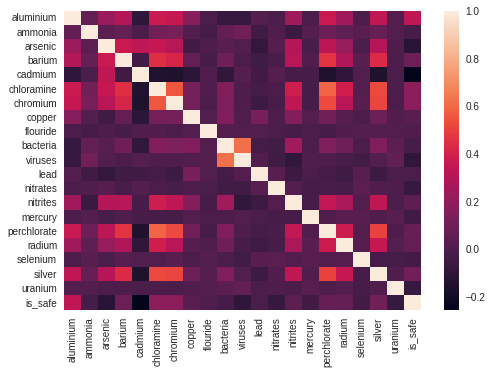
\includegraphics[scale=0.65]{corr1}
\end{center}
Так же построю гистограммы для числовых признаков:
\begin{center}
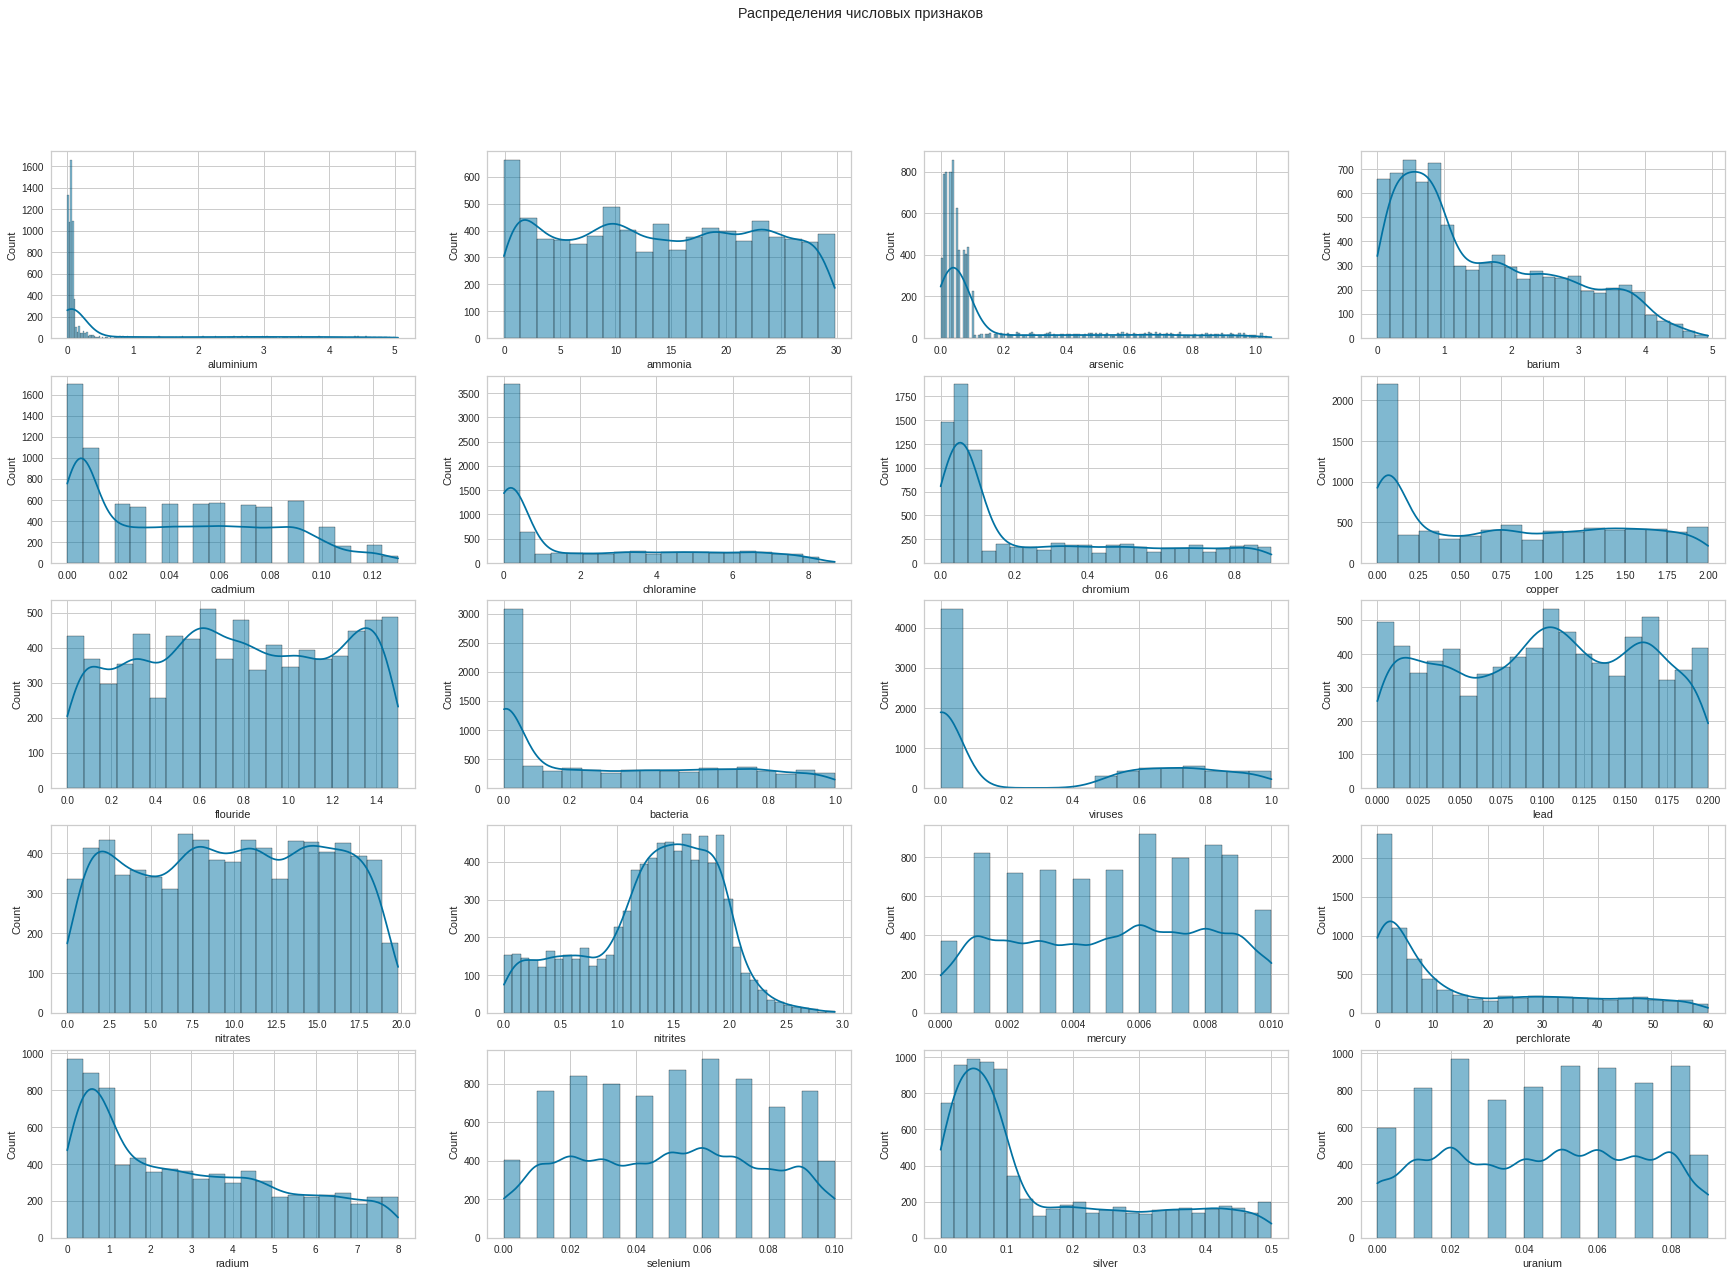
\includegraphics[scale=0.25]{hist1}
\end{center}
Видно, что много признаков распределены плохо. Соотношение классов:
\begin{center}
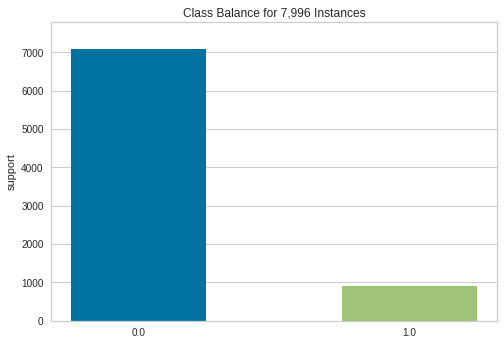
\includegraphics[scale=0.65]{cb1}
\end{center}
Классы несбалансированы, нужно провести аугментацию. Для этого посчитаем матожидание и дисперсию каждого признака, потом сгенерируем нормально распределенные новые признаки по заданным матожиданию и дисперсии.
\pagebreak
Новые распределения:
\begin{center}
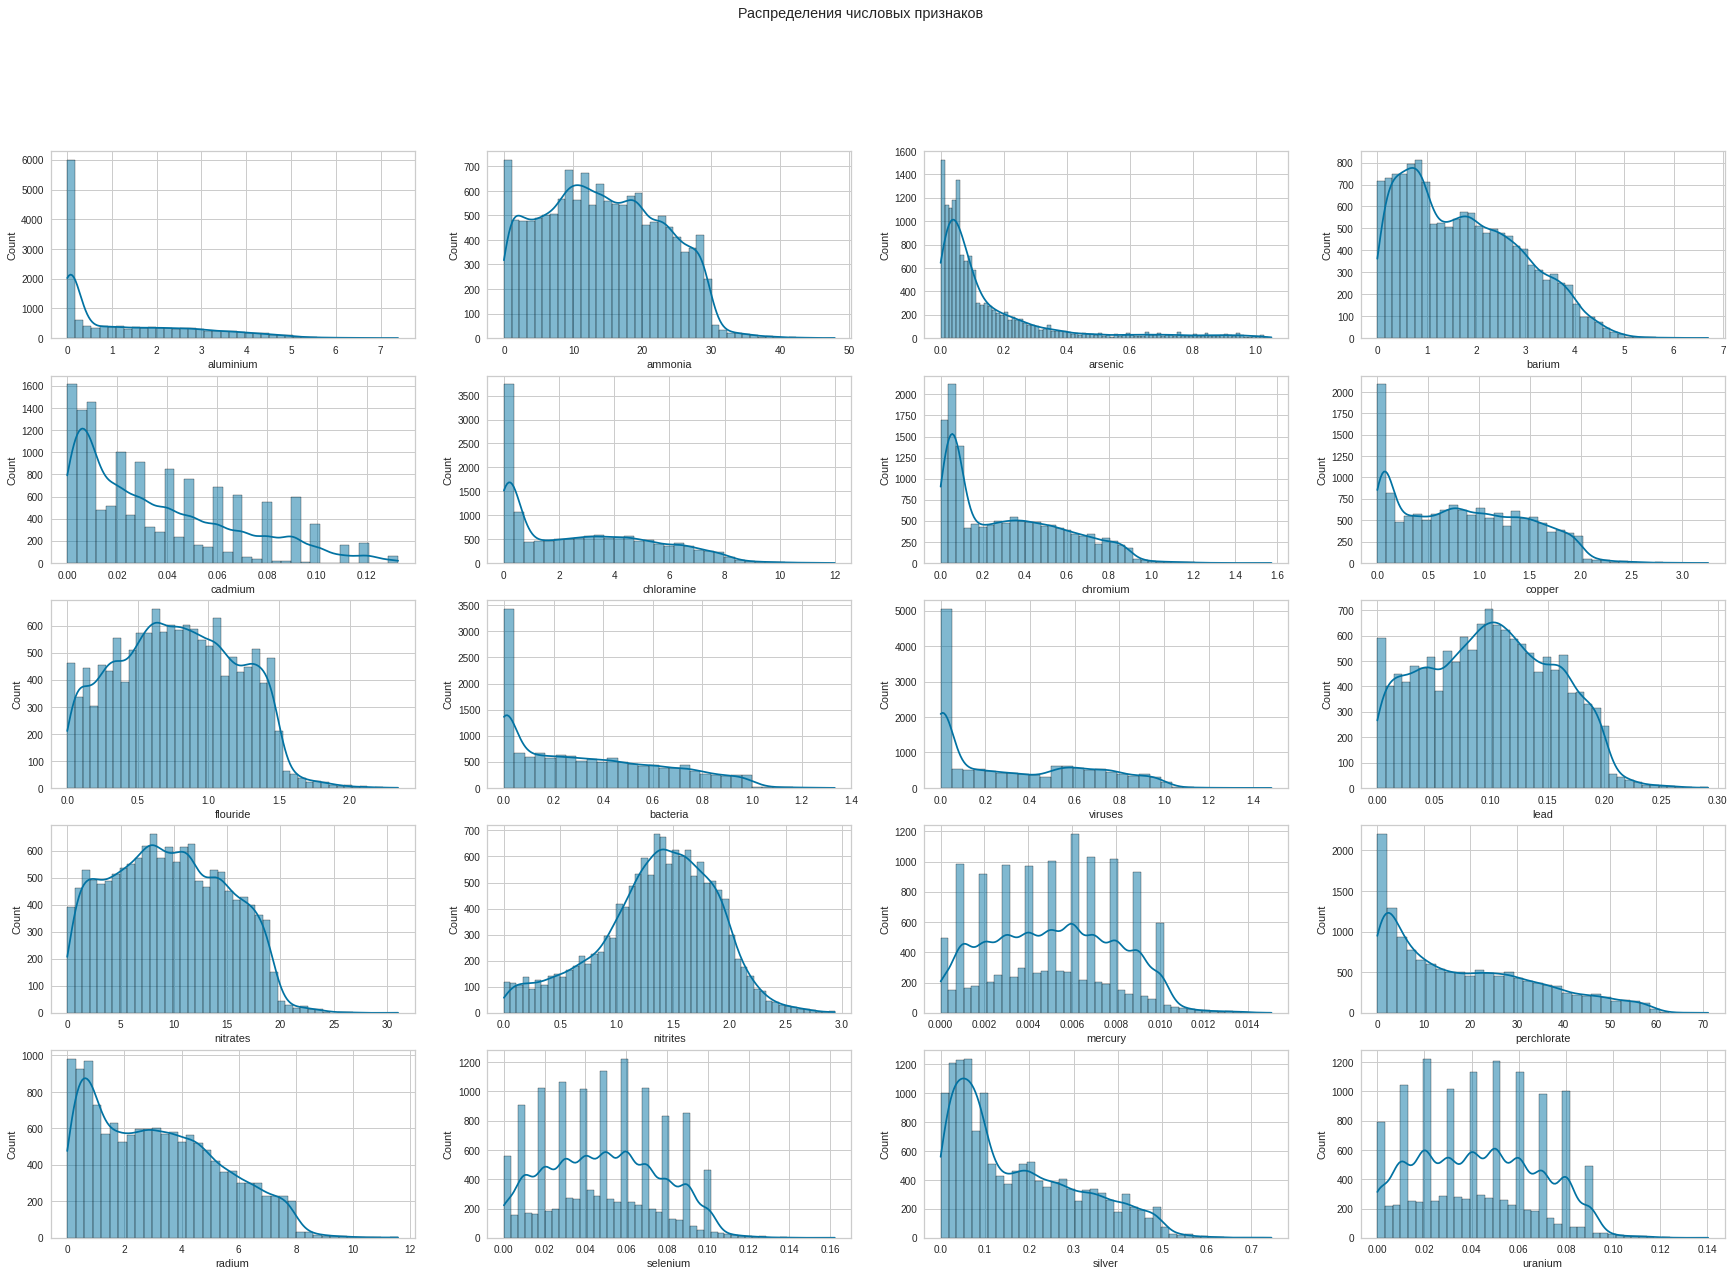
\includegraphics[scale=0.25]{hist2}
\end{center}
Видно, что распределения сильно лучше не стали, однако, забегая вперед, скажу, что такая аугментация повысила recall с 30 процентов до 80-90.
\pagebreak

Корреляционная матрица почти не изменилась:
\begin{center}
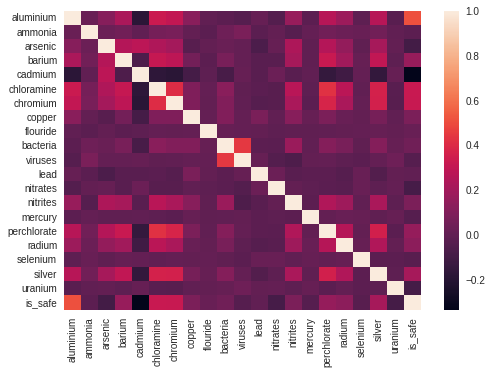
\includegraphics[scale=0.65]{corr2}
\end{center}

Баланс классов:
\begin{center}
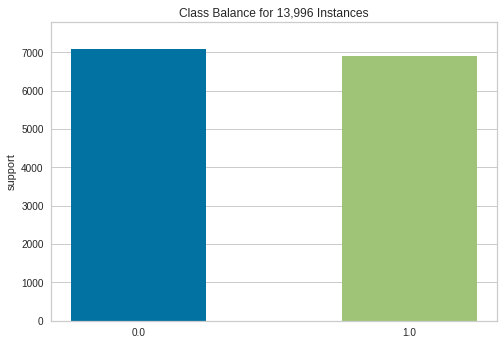
\includegraphics[scale=0.35]{cb2}
\end{center}
Классы стали сбалансированными

\pagebreak
